The solutions of regular ODEs are given as functions of the independent variable time $t$.
Because hybrid automata also include a discrete evolution of the state (namely, via the reset map $\reset$), their solutions will be given as a function of time $t$ and jump number $j$.
We first define hybrid time domains and arcs.
\begin{defn}[Hybrid time domains and arcs~\cite{GoebelT06_SolnsHybInclusions}]
	\label{def:hybridarcs}
	A subset $E \subset \Re_+\times \Ne$ is a \emph{compact hybrid time domain} if 
	\[E = \bigcup_{j=0}^{J-1}[t_j,t_{j+1}]\times \{j\}\]
	for some finite increasing sequence of times $0=t_0 \leq t_1 \leq t_2 \leq \ldots \leq t_J$.
	We say $E$ is a \emph{hybrid time domain} if for all $(T,J) \in E$, 
	$E \cap ([0,T]\times \{0,\ldots,J\})$ is a compact hybrid time domain.
	Define
	$\sup_t E = \sup \{t \sut \exists (t,j) \in E\}$, $\sup_j E = \sup \{j \sut \exists (t,j) \in E\}$,
	and $E.last = (\sup_t E, \sup_j E)$.
	
	A \emph{hybrid arc} $\hstraj$ is a function supported over a hybrid time domain $\hstraj:E \rightarrow \Re^n$, 
	such that for every $j$, $t \mapsto \hstraj(t,j)$ is absolutely continuous in $t$ over $I_j = \{t: (t,j) \in E\}$;
	we call $E$ the domain of $\hstraj$ and write it $\dom \hstraj$.
	%The \emph{graph} of a hybrid arc is the set $\gph \hstraj = \{(t,j,\hstraj(t,j)): (t,j) \in \dom \hstraj\}$.
	Finally, $\dom_t \hstraj = \proj{\dom \hstraj}{\nnreals}$ and $\dom_j \hstraj = \proj{\dom \hstraj}{\Ne}$
\end{defn}

Note that each $I_j$ is an interval.
%$E.last$ indicates the last element of $E$ under the linear order $(t,j) \leq (t',j')$ iff $t \leq t'$ and $j\leq j'$.
As observed in \cite{SanfeliceT10automatica}, hybrid time domains are equivalent to hybrid time trajectories used in \cite{LygerosJSZS03tac} to define executions of hybrid automata.
Output and state trajectories of hybrid automata will be modeled as hybrid arcs. 

Given a hybrid automaton $\Sys$ and a point $\hsPt_0  = (\mode_0, \stPt_0)$, 
a \emph{solution} $\hstraj_{\hsPt_0}$ of $\Sys$ (aka \emph{state trajectory}) is given by a hybrid arc $\hstraj$ 
satisfying the following conditions:
\begin{enumerate}
	\item $\hstraj_{h_0}(0,0) = h_0$
	\item $\hstraj_{h_0}(t,j) = (\mode(t,j),\sttraj(t,j)) \in \hsSet \; \forall (t,j) \in \dom \hstraj$
	\label{item:explicitLX}
	\item For each $j$ s.t. $I_j$ has a non-empty interior, 
	\[\dot{\sttraj}(t,j) \in F_{\mode(t,j)}(\sttraj(t,j))\]
	for almost all $t \in I_j$, and $\sttraj(t,j) \in Inv(\mode(t,j))$ for all $t \in \text{int}I_j$.
	Moreover, 
	\begin{equation*}
	\label{eq:zeroderiv}
	\dot{\mode}(t,j) = 0 \; \forall t \notin \{ \inf I_j, \sup I_j\}
	\end{equation*}
	\label{item:contevolutions}
	\item For all $j$ s.t. $(t,j) \in \dom \hstraj$, $(t,j+1) \in \dom \hstraj$, it holds that $\sttraj(t,j) \in \guard(\mode_i,\mode_k)$ for some $i,k$,
	$\sttraj(t, j+1) = \reset(\sttraj(t,j), (\mode_i,\mode_k))$,
	and $\sttraj(t,j+1) \in Inv(\mode_j)$.
	\label{item:jumpHA}
\end{enumerate}
See Fig.~\ref{fig:HA} for an illustration.
We consider that the discrete time variable $j$ simply counts the location changes (via \eqref{eq:zeroderiv} and Condition \ref{item:jumpHA}).
The transition itself between locations takes 0 real time.
The location changes can only occur when the continuous state $\stPt$ enters a guard set (Condition \ref{item:jumpHA}). 
The sequence of control locations that the trajectory $\hstraj$ visits is denoted by $\loc(\hstraj)$.

If $\hstraj$ is a state trajectory, then $\funcOut \circ \hstraj: \dom \hstraj \rightarrow \hsSet$ is called an \emph{output trajectory}.
We assume that $\funcOut$ is such that an output trajectory is also a hybrid arc, supported on the same hybrid time domain as the corresponding state trajectory:
$\dom \hstraj = \dom \funcOut \circ \hstraj$.

\begin{figure}[tb]
	\centering
	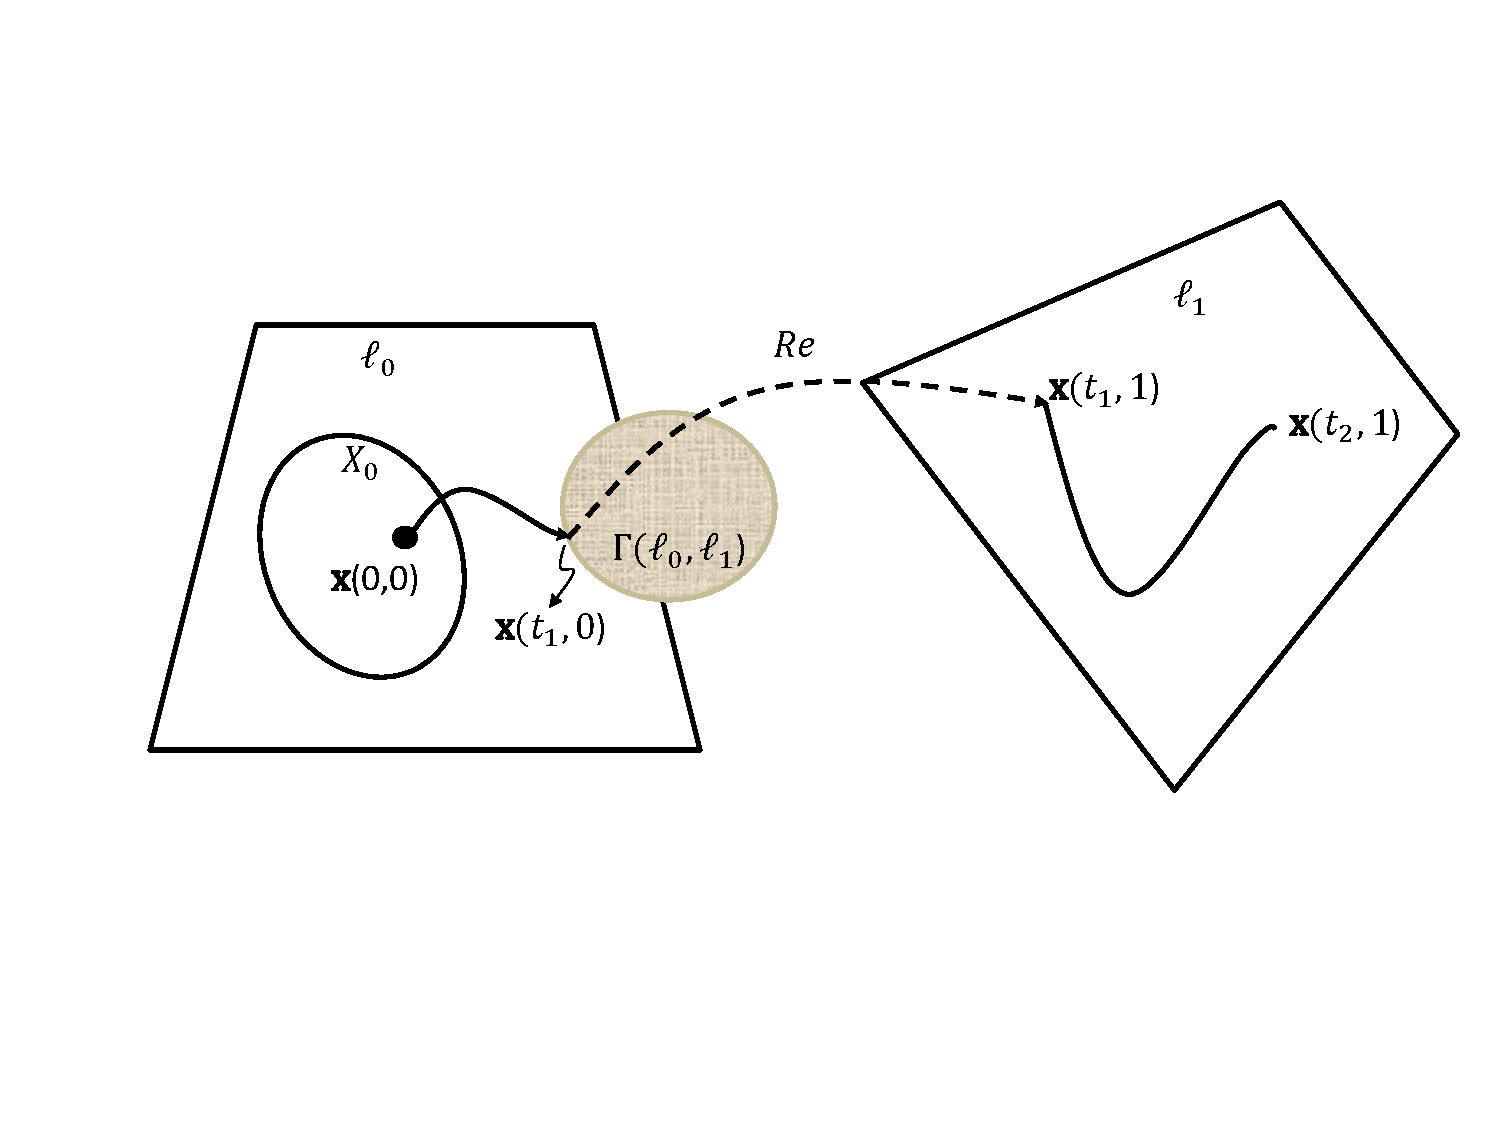
\includegraphics[scale=0.4]{figures/HA.pdf}
	\caption{State trajectory of a hybrid automaton.}
	\label{fig:HA}
\end{figure}

\begin{defn}
	\label{def:solutionsets}
	$\Sc_\Sys(\hsPt_0)$ will denote the set of solutions of $\Sys$ with initial condition $\hstraj(0,0) = \hsPt_0$,
	and $\Sc_\Sys$ will denote the set of all solutions of $\Sys$.
	A hybrid automaton is said to be \emph{deterministic} if $\Sc_\Sys(\hsPt_0)$ is a singleton for any $\hsPt_0$.
\end{defn}

We will use $\hstraj_\hsPt$ to refer to the trajectory starting at $h$.
The system has a finite set of initial locations $\modeSet_0 \subset \modeSet$ in which it could start, 
and within each such location $\mode$, a set of initial continuous states $\stSet_\mode \subset \stSet$ in which it could start. 
Any solution to the system's equations must start there. We denote 
\[H_0 = \bigcup_{\mode \in \modeSet_0} \{\mode\}\times \stSet_\mode\]
the hybrid initial set, and write
\[Init = \bigcup_{\mode \in \modeSet_0}\stSet_\mode \]
